Se propone diseñar un generador de pulsos PWM a partir de la siguiente topología. 

\begin{figure}[H]
    \centering
    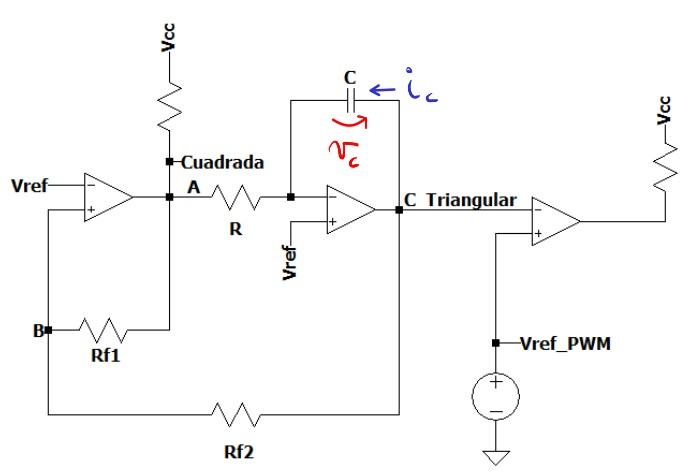
\includegraphics[width=0.8\textwidth]{img/PWM/PWM_topología.jpg}
    \caption{Topología del circuito PWM}
    \label{fig:PWM topologia}
\end{figure}

El circuito consiste en 3 etapas. La etapa 1 es un circuito \textit{Schmitt-trigger} no inversor, el cual generará una señal cuadrada. La segunda etapa es un integrador implementado en un \texttt{OpAmp}, el cual integrará la señal cuadrada para generar una triangular. La última etapa compara la señal triangular con una tensión de referencia variable a través de un potenciómetro. El valor de esta tensión variable permite ajustar el ciclo de trabajo $D$ de los pulsos PWM.

\subsection{Análisis del circuito} 

Es necesario entender cómo varía la frecuencia de las oscilaciones con los componentes para diseñar el circuito. En esta sección, se utilizarán letras minúsculas para las señales variables en el tiempo y letras mayúsculas para las tensiones constantes.

En primer lugar, se buscará la relación entre las señales de los nodos C y A. Al aplicar ley de Ohm a la resistencia $R$ se tiene que $i_c = (V_{ref} -  v_A)/R$, con lo cual

\begin{equation}
    v_c' = i_c/C = -\frac{v_A - V_{ref}}{RC}
\end{equation}

y teniendo en cuenta que $v_{tri} = v_{ref} + v_c$, se llega a 

\begin{equation}
    v_{tri} = -\frac{1}{RC}\int (v_A - V_{ref}) dt + V_{ref}.
    \label{eq:triangular}
\end{equation}

De la \autoref{eq:triangular} se tiene que, si $v_A$ es una señal cuadrada, $v_{tri}$ será una señal triangular montada sobre una tensión continua $V_{ref}$. 

Esta ecuación también indica cómo varían las tensiones del circuito. Si la salida del \textit{Schmitt-trigger} es cero ($v_A = \SI{0}{\volt}$), la tensión $v_{tri}$ crece como una rampa ya que se integra una constante. Eventualmente $v_{tri}$ llegará a un valor lo suficientemente alto para disparar el \textit{Schmitt-trigger}, con lo cual $v_A$ pasará a valer $V_{CC}$. Entonces, la corriente $i_c$ invierte su sentido, el capacitor se descarga y el integrando de la \label{eq:triangular} pasa a ser una constante positiva, por lo que $v_{tri}$ decrece linealmente. Esta tensión decrecerá hasta  llegar al umbral inferior del \textit{Schmitt-trigger}, momento en el cual la tensión $v_A$ volverá a ser cero y el ciclo se repetirá. Este es el principio básico por el cual funciona este circuito.

Para determinar la frecuencia de las oscilaciones es necesario conocer con qué pendiente asciende y desciende la señal triangular, para lo cual se deriva la \autoref{eq:triangular} y se la evalúa en cada semiciclo.

\begin{minipage}{0.45\textwidth}
    \centering
    \begin{equation}
        v_{tri}' = \frac{V_{ref}}{RC} \text{(Subiendo)}
        \label{eq:derivada subiendo}
    \end{equation}
\end{minipage}
\hfill
\begin{minipage}{0.45\textwidth}
    \centering
    \begin{equation}
        v_{tri}' = -\frac{V_
        {CC} - v_{ref}}{RC} \text{(Bajando)}
        \label{eq:derivada bajando}
    \end{equation}
\end{minipage}

Ya que se quiere una señal triangular, las pendientes de subida y bajada deben ser opuestas y de igual módulo. Aplicando estos requerimientos a estas dos ecuaciones se tiene que $V_{ref} = V_{CC}/2$. De esta forma, las pendientes de subida y bajada serán $v_{tri}' = \pm \frac{V_
{CC}}{2RC}$. 

Para determinar la frecuencia de las oscilaciones también es necesario hallar el valor máximo y el valor mínimo de la señal triangular, que se denominarán $V^+$ y $V^-$, respectivamente. De esta forma, cuando $v_A = 0$ la tensión $v_{tri}$ aumenta hasta que $v_{tri} = V^+$, momento en el cual la tensión $V_B$ es igual a $V_{ref}$ y el \textit{Schmitt-trigger} se dispara. Entonces, $v_A$ pasa a valer $V_{CC}$, y la tensión $v_{tri}$ disminuye desde $V^+$ hasta llegar a $V^-$, momento en el cual la tensión $V_B$ es igual a $V_{ref}$ y el \textit{Schmitt-trigger} se vuelve a disparar. 

Para determinar $V^+$ y $V^-$ se busca la tensión del nodo B a partir del divisor resistivo que se forma en las resistencias $R_{f1}$ y $R_{f2}$. Se tiene entonces que

\begin{equation}
    V_B = \frac{R_{f1}}{R_{f1} + R_{f2}} \cdot (v_{tri} - v_A) + v_A.
    \label{eq:nodo B}
\end{equation}

A partir de esta ecuación, se evalúan los dos casos mencionados previamente: cuando $v_A = 0$, $v_{tri} = V^+$ y $V_B = V_{ref}$ y cuando $v_A = V_{CC}$, $v_{tri} = V^-$ y $V_B = V_{ref}$. 

\begin{minipage}{0.45\textwidth}
    \centering
    \begin{equation*}
        V_{ref} = \frac{R_{f1}}{R_{f1} + R_{f2}} \cdot V^+
    \end{equation*}
\end{minipage}
\hfill
\begin{minipage}{0.45\textwidth}
    \centering
    \begin{equation*}
        V_{ref} = \frac{R_{f1}}{R_{f1} + R_{f2}} \cdot (V^- - V_{CC}) + V_{CC}
    \end{equation*}
\end{minipage}

Se despejan entonces $V^+$ y $V^-$ de cada ecuación, teniendo en cuenta que $V_{CC} = 2V_{ref}$ como se estableció previamente.

\begin{minipage}{0.45\textwidth}
    \centering
    \begin{equation}
        V^+ = (1 + \frac{R_{f2}}{R_{f1}}) \cdot V_{ref}
        \label{eq:V+}
    \end{equation}
\end{minipage}
\hfill
\begin{minipage}{0.45\textwidth}
    \centering
    \begin{equation}
        V^- = (1 - \frac{R_{f2}}{R_{f1}}) \cdot V_{ref}
        \label{eq:V-}
    \end{equation}
\end{minipage}


\begin{equation}
    \Delta V = V^+ - V^- = 2 \frac{R_{f2}}{R_{f1}} V_{ref}
    \label{eq:delta V}
\end{equation}
De esta forma, la triangular debe recorrer las tensiones $V^-$ a $V^+$ en la mitad del período, es decir, debe aumentar $\Delta V = V^+ - V^-$ en $T/2$. De las ecuaciones \ref{eq:V+} y \ref{eq:V-} puede obtenerse que $\Delta V = 2 \frac{R_{f2}}{R_{f1}} V_{ref}$. Puede relacionarse el rango de tensiones a recorrer con el tiempo que lleva recorrerlas a través de la derivada (ecuaciones \ref{eq:derivada subiendo} y \ref{eq:derivada bajando}). Se tiene entonces que

\begin{equation*}
    \frac{T}{2} = \frac{\Delta V}{v_{tri}'} = \frac{2 R_{f2}/R_{f1} V_{ref}}{V_{ref}/RC} = 2 RC \frac{R_{f2}}{R_{f1}}. 
\end{equation*}


Se despeja entonces $f = 1/T$.

\begin{equation}
    f = \frac{1}{4RC} \cdot \frac{R_{f1}}{R_{f2}}
    \label{eq:frecuencia}
\end{equation}

\subsection{Diseño y elección de componentes}

En primer lugar, ya que el circuito será alimentado desde una batería cuya tensión podría variar entre $\SI{12}{\volt}$ y $\SI{30}{\volt}$, se eligió un regulador LM7809 para mantener la tensión constante en $\SI{9}{\volt}$ y alimentar al resto del circuito. Esto fija $V_{CC} = \SI{9}{\volt}$ y $V_{ref} = \SI{4,5}{\volt}$. En segundo lugar, se eligió que la amplitud pico a pico de la señal triangular fuera de \SI{1}{\volt}, con lo cual de la \autoref{eq:delta V} se tiene que

\begin{equation*}
    \frac{R_{f2}}{R_{f1}} = \frac{1}{9}.
\end{equation*}

En principio se eligieron $R_{f1} = \SI{510}{\kilo \Omega}$ y $R_{f2} = \SI{56}{\kilo \Omega}$, pero finalmente se usaron $R_{f1} = \SI{560}{\kilo \Omega}$ y $R_{f2} = \SI{56}{\kilo \Omega}$ ya que no fue posible adquirir resistores de los valores originales. 

Luego, se busca una frecuencia de trabajo de aproximadamente \SI{135}{\kilo \hertz}. Se eligió un capacitor de \SI{120}{\pico \farad} y se despejó la resistencia $R$ de la \autoref{eq:frecuencia}, dando un valor de $R = \SI{154,3}{\kilo \Omega}$, cuyo valor comercial más cercano es $\SI{150}{\kilo \Omega}$. Estos valores dan, finalmente, una frecuencia de oscilación de $f = \SI{138,8}{\kilo \hertz}$.

Para el amplificador operacional se utilizó el integrado TL072, el cual presenta un slew rate lo suficientemente grande para esta aplicación. Además, es un circuito específicamente diseñado para minimizar el ruido, lo que lo hace preferible por sobre otros amplificadores de la familia TL0XX. En el encapsulado se incluyen 2 amplificadores, uno de los cuales fue utilizado como integrador. El segundo fue utilizado para generar la tensión $V_{ref} = \SI{4,5}{\volt}$ con un divisor resistivo y un seguidor. 

Para el comparador se eligió el LM393, de amplia disponibilidad y con requisitos suficientes para esta aplicación. Se procuró usar un comparador lo suficientemente rápido para la frecuencia de trabajo y que pudiera alcanzar todo el rango de tensiones. 

Según la hoja de datos del LM393, la corriente máxima que puede ingresar al comparador es $I_{MAX} = \SI{1,5}{\ampere}$. Es necesario, entonces, poner resistencias de \textit{pull-up} para limitar esta corriente. La resistencia de \textit{pull-up} mínima es $R_{PU} = V_{CC}/I_{MAX} = \SI{1,5}{\kilo \Omega}$, pero se optó por resistencias de $\SI{5,1}{\kilo \Omega}$ ya que mejoraban el desempeño del circuito. 

\subsection{Simulación y diseño del PCB}

\begin{figure}[H]
    \centering
    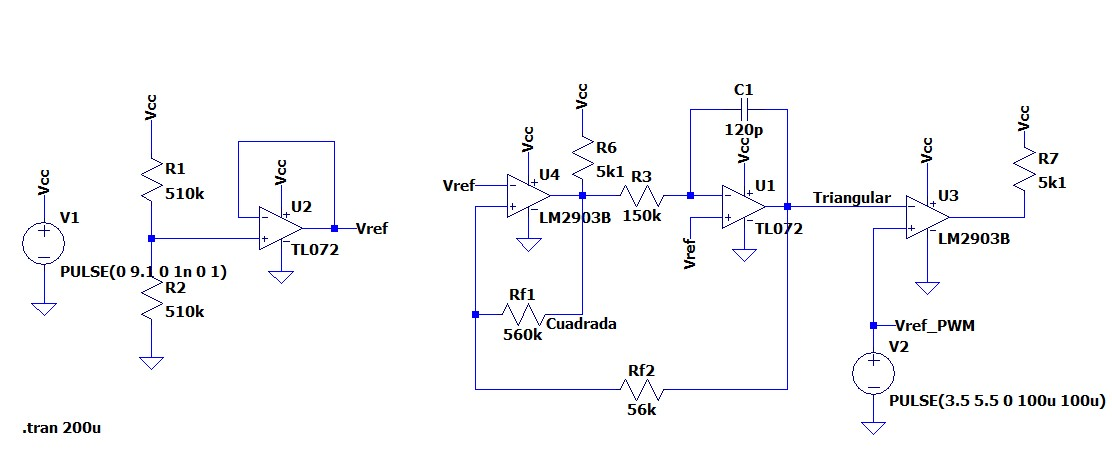
\includegraphics[width=0.8\textwidth]{img/PWM/PWM_simulación.jpg}
    \caption{Simulación en \textit{LTSpice}}
    \label{fig:circuito simulacion}
\end{figure}

Se utilizó el circuito de la \autoref{fig:circuito simulacion} para simular el PWM en \textit{LTSpice}. Los resultados pueden verse en la \autoref{fig:señales}.


\begin{figure}[H]
    \centering
    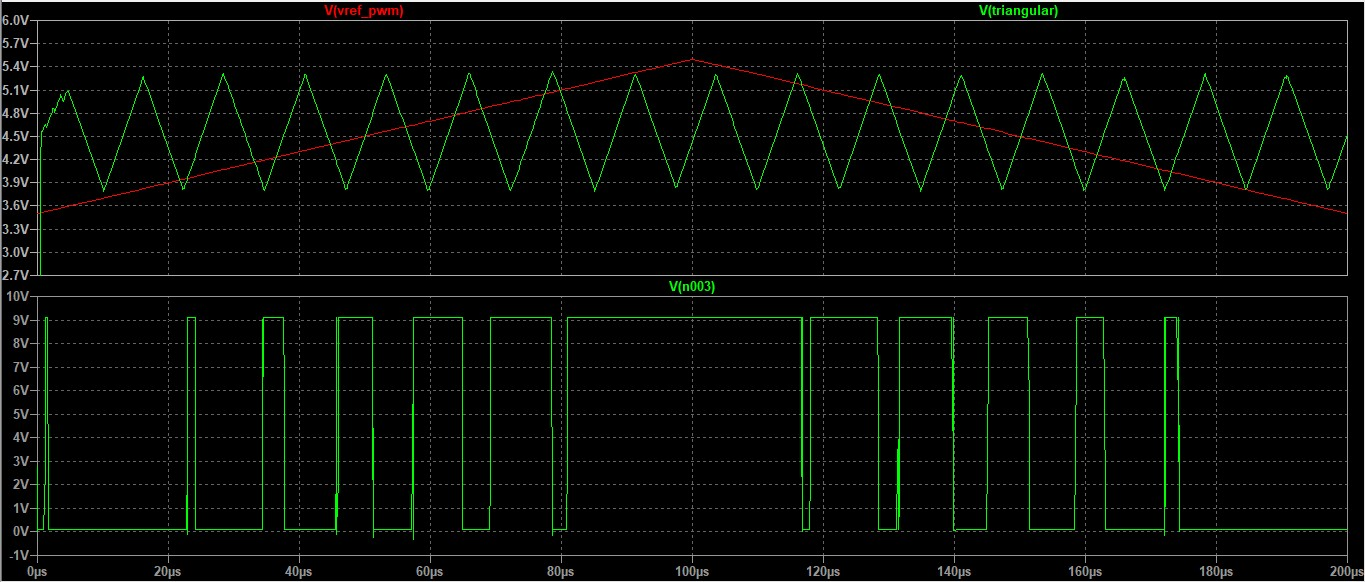
\includegraphics[width=0.95\textwidth]{img/PWM/PWM_señales.jpg}
    \caption{Resultados de la simulación}
    \label{fig:señales}
\end{figure}

Puede apreciarse que el PWM funciona según lo esperado, excepto por la frecuencia de oscilación, la cual es $f = \SI{80}{\kilo \hertz}$. Se decidió entonces reemplazar el capacitor C de $\SI{120}{\pico \farad}$ por uno más chico de $\SI{47}{\pico \farad}$. 

La causa de esta discrepancia es el modelo del comparador y su tiempo de respuesta. El tiempo de respuesta es el tiempo que tardan en propagarse los cambios en la entrada a la salida. Es decir, ante un cambio en las entradas del comparador, el cambio correspondiente en la salida solo se hará efectivo un tiempo de respuesta luego. Según su hoja de datos, el LM393 presenta un tiempo de respuesta de $\SI{1,3}
{\micro s}$, lo que resulta comparable con el período de la señal y explica que las oscilaciones sean más lentas. 

\begin{figure}[H]
    \centering
    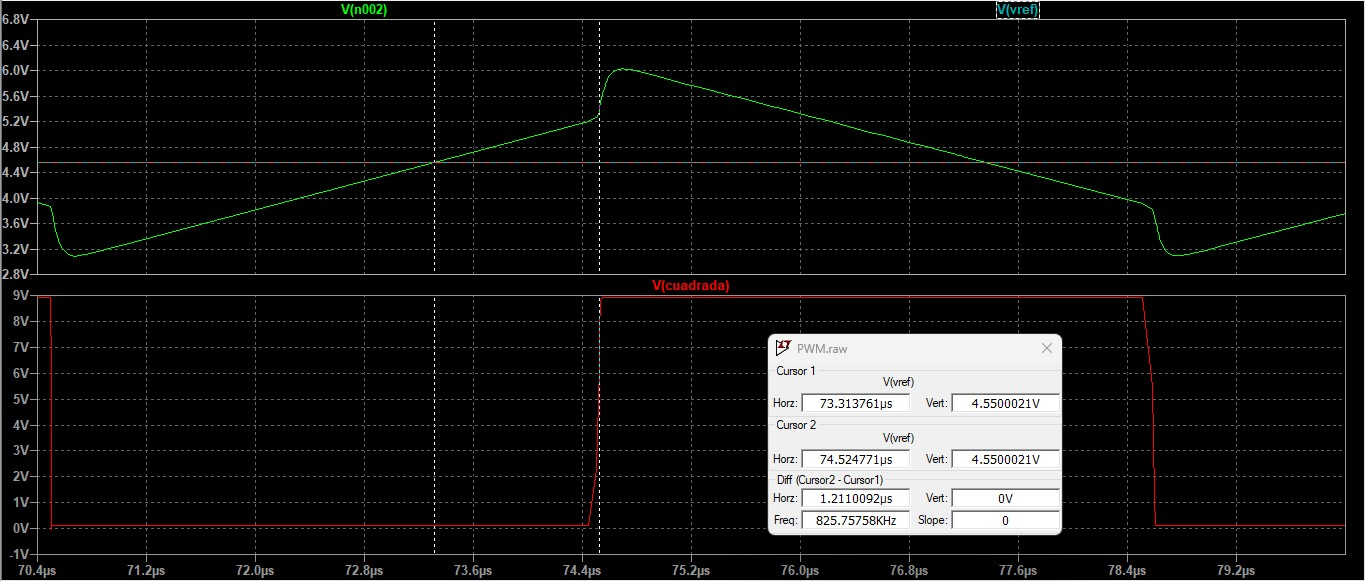
\includegraphics[width=0.95\textwidth]{img/PWM/Tiempo de respuesta.jpg}
    \caption{Tiempo de respuesta del comparador}
    \label{fig:tiempo de respuesta}
\end{figure}

En la \autoref{fig:tiempo de respuesta} puede observarse que el tiempo de respuesta del comparador es de aproximadamente $\SI{1,2}{\micro s}$ en la simulación. Las dos imágenes en el panel superior son las entradas del comparador. Vemos que cuando se cruzan, la salida del comparador no cambia instantáneamente. También se observa en la simulación que la salida del comparador no llega a los valores de la alimentación ($V_{CC}$ y \texttt{GND}). Si bien se acerca bastante, esto es otra fuente de discrepancias ya que no fue considerada en el análisis teórico. Estos dos efectos tienden a hacer al circuito más lento, lo que explica la necesidad de un nuevo capacitor.


Con el circuito ya simulado, se diseñó y construyó el PCB. 

\begin{figure}[H]
    \centering
    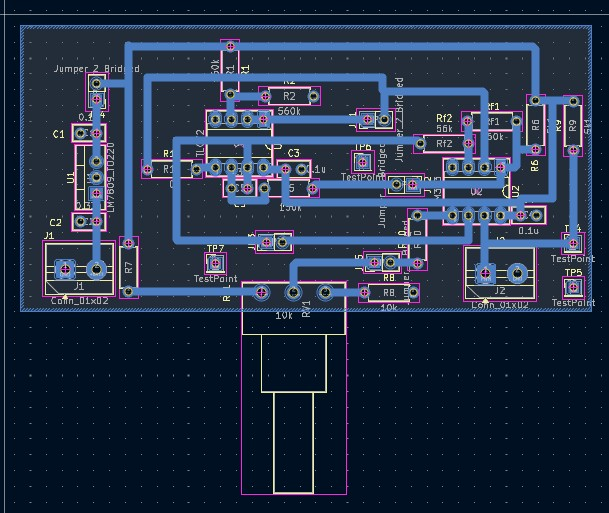
\includegraphics[width=0.8\textwidth]{img/PWM/PWM PCB.jpg}
    \caption{PCB diseñado}
    \label{fig:PCB}
\end{figure}

\begin{figure}[H]
    \centering
    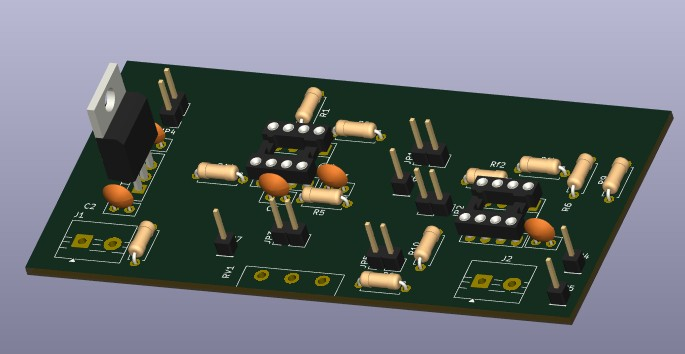
\includegraphics{img/PWM/PWM PCB3D.jpg}
    \caption{PCB diseñado}
    \label{fig:PCB 3D}
\end{figure}

\subsection{Mediciones}

Con el circuito ya armado se midieron las señales del circuito con un osciloscopio. Fue necesario configurar la punta y el equipo en \texttt{X10} para que la punta no filtrara los armónicos de las frecuencias más elevadas. 

En un primer momento se observó que la frecuencia de las oscilaciones era excesivamente alta ($f = \SI{200}{\kilo \hertz}$), por lo que nuevamente se ajustó el valor del capacitor a uno de $\SI{100}{\pico \farad}$, lo que redujo la frecuencia a $f = \SI{118}{\kilo \hertz}$. Hecho este cambio, se hicieron mediciones con el osciloscopio para obtener los siguientes gráficos. 

\begin{minipage}{0.45\textwidth}
    \centering
    \begin{figure}[H]
        \centering
        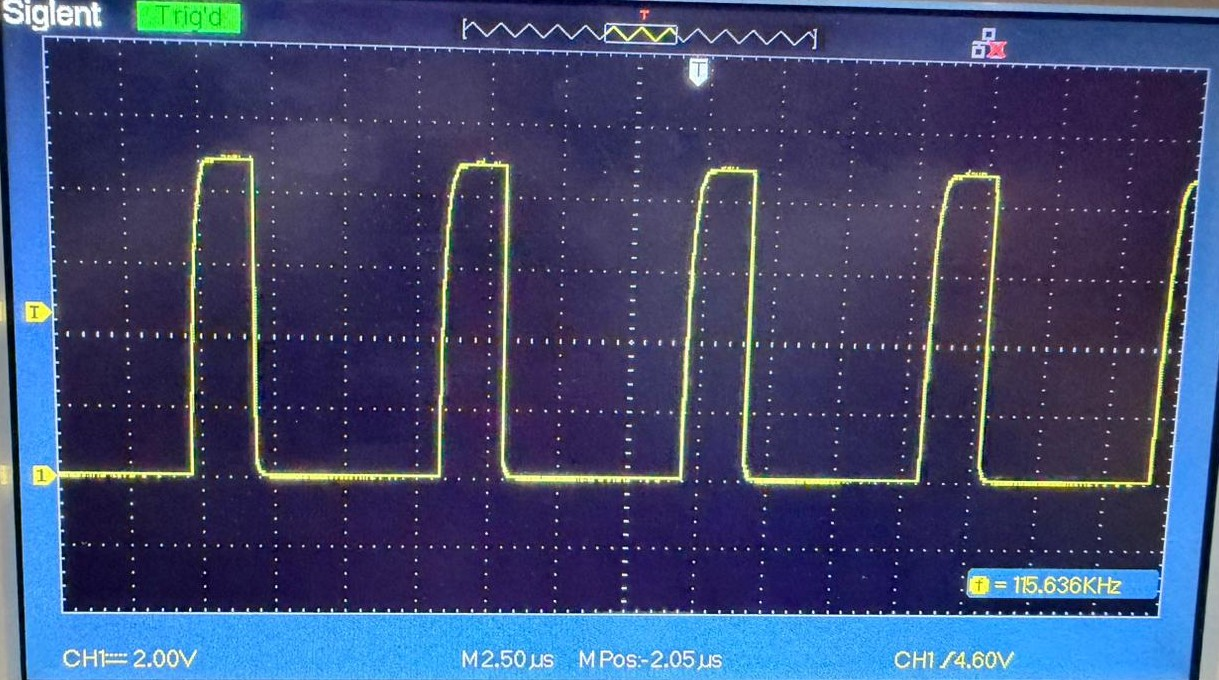
\includegraphics[width=0.9\textwidth]{img/PWM/DC_chico.jpeg}
        \caption{Salida con \textit{duty cycle} menor}
        \label{fig:DC chico}
    \end{figure}
\end{minipage}
\hfill
\begin{minipage}{0.45\textwidth}
    \centering
    \begin{figure}[H]
        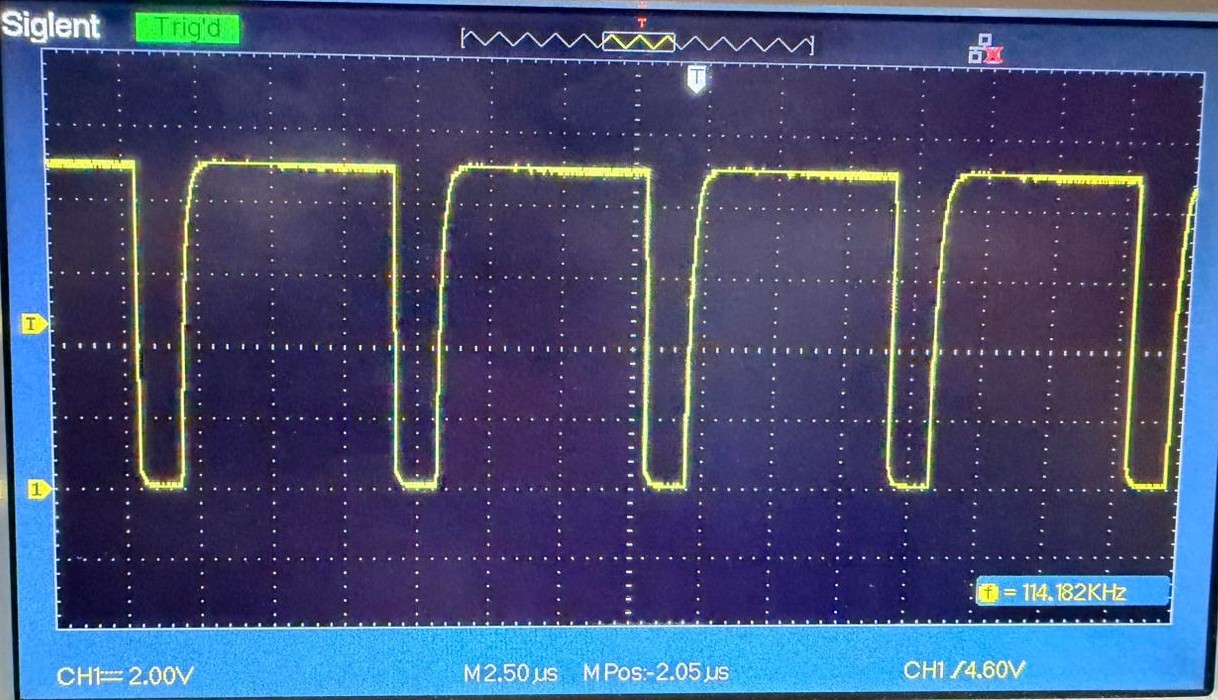
\includegraphics[width=0.9\textwidth]{img/PWM/DC_grande.jpeg}
        \caption{Salida con \textit{duty cycle} mayor}
        \label{fig:DC grande}
    \end{figure}
\end{minipage}

\begin{figure}[H]
    \centering
    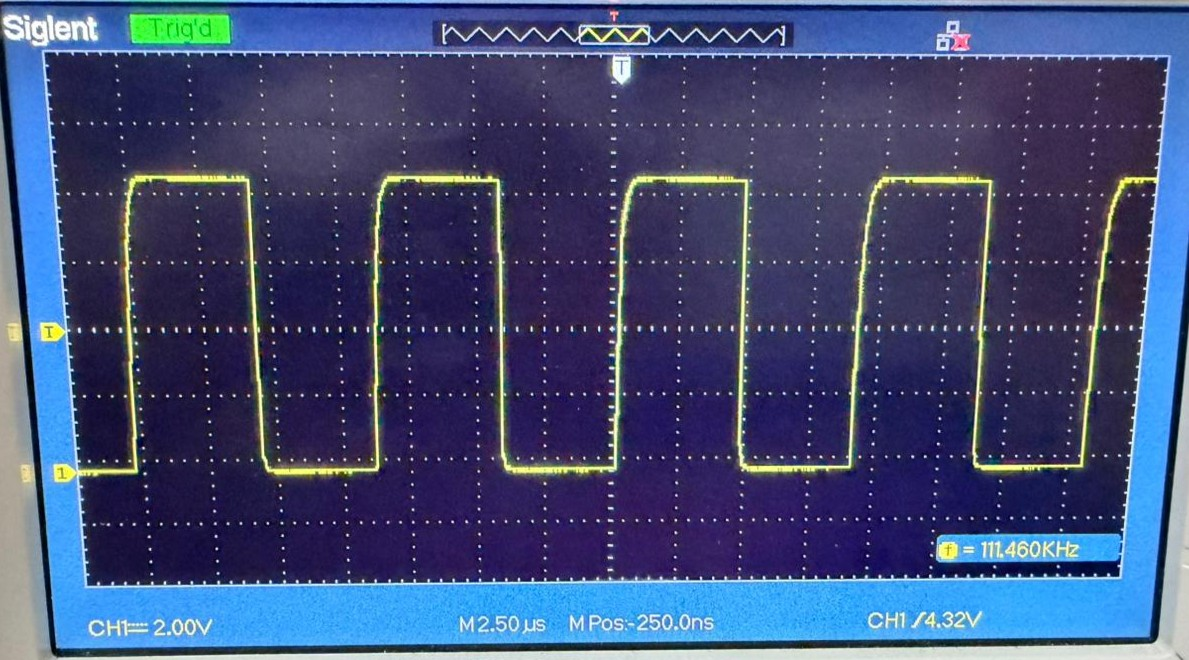
\includegraphics[width=0.9\textwidth]{img/PWM/Cuadrada.jpeg}
    \caption{Señal cuadrada}
    \label{fig:Cuadrada}
\end{figure}

\begin{figure}[H]
    \centering
    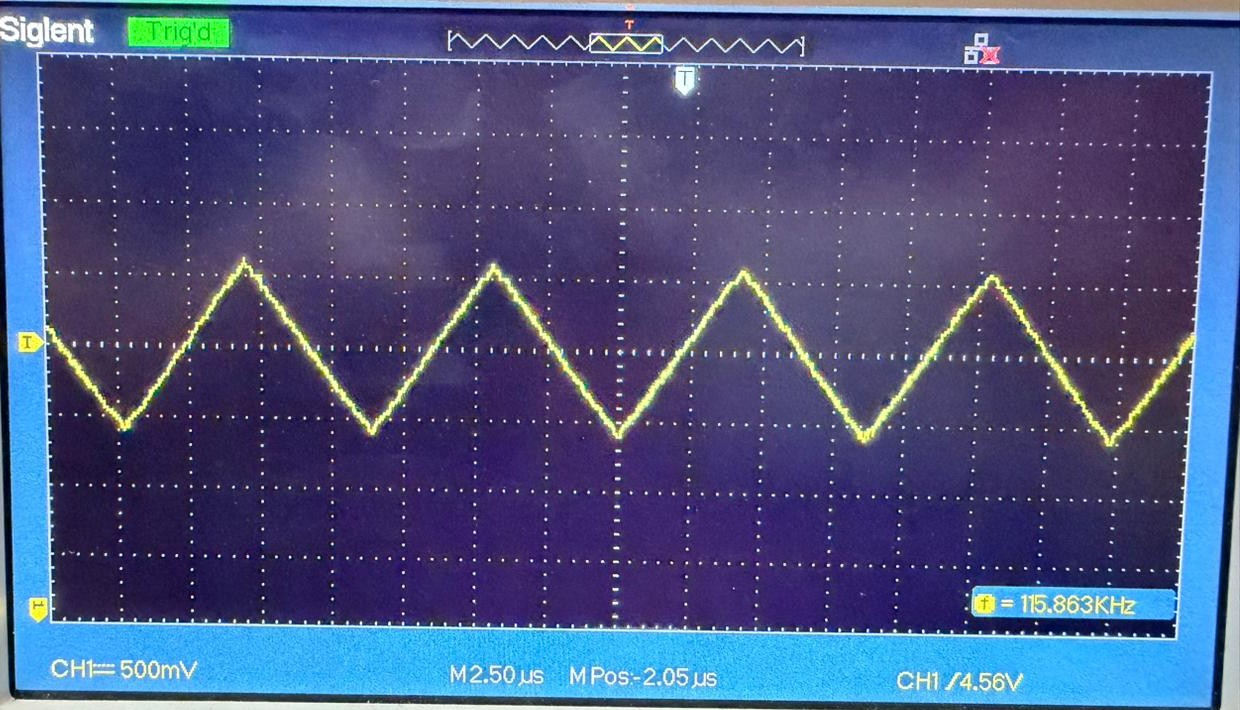
\includegraphics[width=0.9\textwidth]{img/PWM/Triangular.jpeg}
    \caption{Señal triangular}
    \label{fig:triangular}
\end{figure}
